% ============================================================
%  طرح پیشنهادی مجلس مهستان — نسخه‌ی خلاصه‌ی اجرایی
%  کامپایل: XeLaTeX (دو بار)
%  فونت: Vazirmatn
% ============================================================
\documentclass[a4paper,11pt]{article}

% ---------- بسته‌های پایه ----------
\usepackage[top=1.8cm, bottom=2cm, left=2cm, right=2cm]{geometry}
\usepackage{fontspec}
\usepackage{graphicx}
\usepackage{xcolor}
\usepackage{tikz}
\usetikzlibrary{%
	shapes.geometric,%
	arrows.meta,%
	positioning,%
	calc,%
	backgrounds,%
	fit,%
	shadows.blur%
}
\usepackage{tcolorbox}
\tcbuselibrary{skins, breakable}
\usepackage{tabularx}
\usepackage{booktabs}
\usepackage{enumitem}
\usepackage{fancyhdr}
\usepackage{hyperref}
\usepackage{amssymb}
\usepackage{colortbl}
\usepackage{array}
\usepackage{ragged2e}
\usepackage{setspace}
\usepackage{titlesec}
\usepackage{lastpage}
\usepackage{needspace}
\usepackage{adjustbox}

% ---------- تعریف رنگ‌ها ----------
\definecolor{mahestan-blue}{HTML}{1565C0}
\definecolor{mahestan-green}{HTML}{2E7D32}
\definecolor{mahestan-gold}{HTML}{F9A825}
\definecolor{mahestan-red}{HTML}{C62828}
\definecolor{mahestan-purple}{HTML}{6A1B9A}
\definecolor{mahestan-orange}{HTML}{E65100}
\definecolor{mahestan-teal}{HTML}{00838F}
\definecolor{bg-light-blue}{HTML}{E3F2FD}
\definecolor{bg-light-green}{HTML}{E8F5E9}
\definecolor{bg-light-gold}{HTML}{FFF9C4}
\definecolor{bg-light-red}{HTML}{FFEBEE}
\definecolor{bg-light-purple}{HTML}{F3E5F5}
\definecolor{bg-cream}{HTML}{FFFDE7}
\definecolor{bg-gray}{HTML}{F5F5F5}
\definecolor{border-gray}{HTML}{BDBDBD}
\definecolor{text-dark}{HTML}{212121}
\definecolor{text-medium}{HTML}{424242}

% ---------- هایپرلینک ----------
\hypersetup{
	colorlinks=true,
	linkcolor=mahestan-blue,
	urlcolor=mahestan-teal,
	pdfencoding=unicode,
	pdfTitle={طرح پیشنهادی مجلس مهستان},
	pdfsubject={چارچوب نهادی گذار دموکراتیک ایران},
}

% ---------- باکس‌ها ----------
\newtcolorbox{tocbox}{%
	enhanced,
	breakable,
	colback=bg-light-blue,
	colframe=mahestan-blue,
	boxrule=1.2pt,
	arc=6pt,
	left=10pt, right=10pt, top=10pt, bottom=10pt,
	before skip=12pt,
	after skip=12pt,
	shadow={2pt}{-2pt}{0pt}{black!15}%
}

\newtcolorbox{principlebox}[1][]{%
	enhanced,
	breakable,
	colback=bg-light-blue,
	colframe=mahestan-blue,
	coltitle=white,
	fonttitle=\bfseries\large,
	boxrule=1.5pt,
	arc=4pt,
	left=8pt, right=8pt, top=6pt, bottom=6pt,
	before skip=12pt,
	after skip=12pt,
	shadow={2pt}{-2pt}{0pt}{black!20},
	#1%
}

\newtcolorbox{alertbox}[1][]{%
	enhanced,
	breakable,
	colback=bg-light-red,
	colframe=mahestan-red,
	coltitle=white,
	fonttitle=\bfseries,
	boxrule=1.5pt,
	arc=4pt,
	left=8pt, right=8pt, top=6pt, bottom=6pt,
	before skip=12pt,
	after skip=12pt,
	#1%
}

\newtcolorbox{quotebox}[1][]{%
	enhanced,
	breakable,
	colback=bg-cream,
	colframe=mahestan-gold,
	boxrule=0pt,
	borderline west={3pt}{0pt}{mahestan-gold},
	left=12pt, right=8pt, top=6pt, bottom=6pt,
	sharp corners,
	before skip=12pt,
	after skip=12pt,
	#1%
}

\newtcolorbox{greenbox}[1][]{%
	enhanced,
	breakable,
	colback=bg-light-green,
	colframe=mahestan-green,
	coltitle=white,
	fonttitle=\bfseries,
	boxrule=1.5pt,
	arc=4pt,
	left=8pt, right=8pt, top=6pt, bottom=6pt,
	before skip=12pt,
	after skip=12pt,
	#1%
}

% ---------- عنوان‌ها ----------
\titleformat{\section}
{\color{mahestan-blue}\bfseries\Large}
{\thesection.}{0.5em}{}

\titlespacing*{\section}{0pt}{18pt}{8pt}

\titleformat{\subsection}
{\color{mahestan-purple}\bfseries\large}
{\thesubsection.}{0.5em}{}

\titlespacing*{\subsection}{0pt}{12pt}{6pt}

\titleformat{\subsubsection}
{\color{mahestan-green}\bfseries\normalsize}
{\thesubsubsection.}{0.5em}{}

\titlespacing*{\subsubsection}{0pt}{8pt}{4pt}

% ---------- سربرگ و پابرگ ----------
\pagestyle{fancy}
\fancyhf{}
\renewcommand{\headrulewidth}{1pt}
\renewcommand{\headrule}{%
	\hbox to\headwidth{%
		\color{mahestan-blue}\leaders\hrule height \headrulewidth\hfill}}
\renewcommand{\footrulewidth}{0.5pt}
\renewcommand{\footrule}{%
	\hbox to\headwidth{%
		\color{border-gray}\leaders\hrule height \footrulewidth\hfill}}

% ---------- xepersian آخرین بسته ----------
\usepackage{xepersian}
\settextfont[Scale=1.05]{Vazirmatn}
\setdigitfont{Vazirmatn}
\setlatintextfont[Scale=0.95]{Vazirmatn}
%\DefaultMathsDigits

\fancyhead[R]{%
	\small\textcolor{mahestan-blue}{\textbf{طرح پیشنهادی مجلس مهستان}}}
\fancyhead[L]{%
	\small\textcolor{text-medium}{نسخه‌ی خلاصه‌ی اجرایی}}
\fancyfoot[C]{%
	\small\textcolor{text-medium}{صفحه‌ی \thepage\ از \pageref{LastPage}}}
\fancyfoot[L]{%
	\tiny\textcolor{border-gray}{اسفند ۱۴۰۴}}

% ============================================================
\begin{document}
	\setstretch{1.3}
	
	% ==================== صفحه‌ی عنوان ====================
	\thispagestyle{empty}
	
	\begin{tikzpicture}[remember picture, overlay]
		\fill[mahestan-blue]
		(current page.north west) rectangle
		([yshift=-9cm]current page.north east);
		\fill[mahestan-gold]
		([yshift=-9cm]current page.north west) rectangle
		([yshift=-9.4cm]current page.north east);
		\fill[mahestan-green!70]
		([yshift=-9.4cm]current page.north west) rectangle
		([yshift=-9.6cm]current page.north east);
		\fill[mahestan-blue!10]
		(current page.south west) rectangle
		([yshift=2.5cm]current page.south east);
		\fill[mahestan-gold]
		([yshift=2.5cm]current page.south west) rectangle
		([yshift=2.7cm]current page.south east);
	\end{tikzpicture}
	
	\vspace*{1.5cm}
	
	\begin{center}
		{\Huge\textcolor{white}{\textbf{طرح پیشنهادی}}}\\[0.3cm]
		{\fontsize{36}{42}\selectfont\textcolor{white}{\textbf{مجلس مهستان}}}\\[0.5cm]
		{\Large\textcolor{bg-light-blue}{چارچوب نهادی گذار دموکراتیک ایران}}
	\end{center}
	
	\vspace{3cm}
	
	\begin{center}
		\begin{tcolorbox}[
			enhanced,
			width=12cm,
			colback=bg-cream,
			colframe=mahestan-gold,
			boxrule=2pt,
			arc=8pt,
			halign=center,
			before skip=12pt,
			after skip=12pt,
			shadow={3pt}{-3pt}{0pt}{black!15}
			]
			{\large\textbf{نسخه‌ی خلاصه‌ی اجرایی}}\\[0.3cm]
			{\normalsize ایران برای همه‌ی ایرانیان}\\[0.3cm]
			{\small\textcolor{text-medium}{اسفند ۱۴۰۴ / فوریه‌ی ۲۰۲۶}}
		\end{tcolorbox}
	\end{center}
	
	\vspace{2cm}
	
	\begin{center}
		\textcolor{mahestan-purple}{\rule{14cm}{0.5pt}}\\[0.5cm]
		{\small\textcolor{text-medium}{%
				این سند زنده است و با مشارکت همگان بهتر خواهد شد.\\
				تمام اعداد و نسبت‌ها پیشنهادی هستند و توسط مجلس منتخب مردم نهایی خواهند شد.}}
	\end{center}
	
	\newpage
	
	% ==================== فهرست مطالب ====================
	\thispagestyle{fancy}
	
	\needspace{6\baselineskip}
	\nopagebreak[4]%
	
	
	\begin{tocbox}
		\begin{center}
			{\large\bfseries\textcolor{mahestan-blue}{فهرست مطالب}}
		\end{center}
		\setlength{\tabcolsep}{6pt}%
		\begin{center}
			\begin{tabularx}{\textwidth} { 
					>{\centering\arraybackslash}p{20mm} 
					>{\raggedleft\arraybackslash}X 
					>{\centering\arraybackslash}p{20mm}
				}
				\toprule[1.5pt]
				\rowcolor{bg-light-blue}
				\textcolor{mahestan-blue}{\centering\bfseries بخش} &
				\textcolor{mahestan-blue}{\centering\bfseries موضوع} &
				\textcolor{mahestan-blue}{\centering\bfseries صفحه} \\
				\midrule
				۱ & چرایی و ضرورت طرح مهستان & ۲ \\
				\rowcolor{bg-gray}
				۲ & شش اصل راهنمای طراحی & ۲ \\
				۳ & ساختار مجلس مهستان و ترکیب آن & ۳ \\
				\rowcolor{bg-gray}
				۴ & نهادهای کلیدی دوران گذار و عدالت انتقالی & ۳ \\
				۵ & اولویت‌های ۱۰۰ روز نخست & ۴ \\
				\rowcolor{bg-gray}
				۶ & اصول بنیادین غیرقابل‌نقض & ۴ \\
				۷ & نقشه‌ی راه زمانی & ۵ \\
				\rowcolor{bg-gray}
				۸ & فراخوان مشارکت & ۵ \\
				\bottomrule	
				
			\end{tabularx}
		\end{Center}
	\end{tocbox}
	
	\vspace{0.2cm}
	
	% ==================== بخش ۱ ====================
	\needspace{3\baselineskip}
	\section{\rl{چرایی و ضرورت}}
	
	\begin{quotebox}
		{\itshape\rl{%
				«کیفیت طراحی نهادی دوران گذار، بیش از هر عامل دیگری،
				سرنوشت نظام سیاسی آینده را تعیین می‌کند.»}}
	\end{quotebox}
	
	\vspace{0.3cm}
	
	ایران در مقطعی تاریخی قرار دارد. تجربه‌ی جهانی یک درس بنیادین دارد:
	
	\vspace{0.5\baselineskip}
	\begin{center}
		\begin{adjustbox}{max width=\linewidth}
			\begin{tikzpicture}
				\node[draw=mahestan-green, fill=bg-light-green, rounded corners=6pt,
				minimum width=7cm, minimum height=1.4cm, text width=6.5cm,
				align=center, font=\small\bfseries]
				(success) {%
					\rl{گذار طراحی‌شده + فراگیر}%
					\quad$\longrightarrow$\quad%
					\rl{دموکراسی پایدار}\\%
					{\footnotesize\textcolor{text-medium}{%
							\rl{آفریقای جنوبی {\textperiodcentered} اسپانیا {\textperiodcentered} شیلی {\textperiodcentered} لهستان}}}};
				\node[draw=mahestan-red, fill=bg-light-red, rounded corners=6pt,
				minimum width=7cm, minimum height=1.4cm, text width=6.5cm,
				align=center, font=\small\bfseries, below=0.5cm of success]
				(fail) {%
					\rl{گذار شتاب‌زده + حذفی}%
					\quad$\longrightarrow$\quad%
					\rl{هرج‌ومرج یا استبداد نو}\\%
					{\footnotesize\textcolor{text-medium}{%
							\rl{لیبی {\textperiodcentered} مصر {\textperiodcentered} عراق}}}};
			\end{tikzpicture}
		\end{adjustbox}
	\end{center}
	\vspace{0.5\baselineskip}
	
	مردم ایران --- از هر قشر و طبقه --- هزینه‌های گزافی پرداخت کرده‌اند.
	آینده باید با \textbf{اندیشه، اجماع و مهندسی نهادی} ساخته شود؛
	نه با تعلل و ترس از تغییر، و نه با شتاب و تمامیت‌خواهی.
	
	% ==================== بخش ۲ ====================
	\needspace{6\baselineskip}
	\section{\rl{شش اصل راهنمای طراحی}}
	
	\vspace{0.5\baselineskip}
	\begin{center}
		\begin{adjustbox}{max width=\linewidth}
			\begin{tikzpicture}[
				principle/.style n args={1}{
					draw=#1, fill=#1!8, rounded corners=5pt,
					minimum width=4.6cm, minimum height=1.6cm,
					text width=4.2cm, align=center, font=\small,
					blur shadow={shadow blur steps=5,
						shadow xshift=1pt, shadow yshift=-1pt}
				}
				]
				\node[principle={mahestan-blue}] (p1) at (0,0)
				{\textbf{\textcolor{mahestan-blue}{\rl{اصل ۱}}}\\%
					\rl{ترکیب دموکراسی}\\%
					\rl{مستقیم و تخصص‌گرایی}};
				\node[principle={mahestan-green}] (p2) at (5.3,0)
				{\textbf{\textcolor{mahestan-green}{\rl{اصل ۲}}}\\%
					\rl{نمایندگی نسبتی}\\%
					\rl{هیچ صدایی نشنیده نماند}};
				\node[principle={mahestan-purple}] (p3) at (10.6,0)
				{\textbf{\textcolor{mahestan-purple}{\rl{اصل ۳}}}\\%
					\rl{قانون‌اساسی‌گرایی}\\%
					\rl{دو مرحله‌ای (موقت + نهایی)}};
				\node[principle={mahestan-orange}] (p4) at (0,-2.5)
				{\textbf{\textcolor{mahestan-orange}{\rl{اصل ۴}}}\\%
					\rl{اصلاح نه تخریب}\\%
					\rl{حفظ نهادها با رهبری جدید}};
				\node[principle={mahestan-teal}] (p5) at (5.3,-2.5)
				{\textbf{\textcolor{mahestan-teal}{\rl{اصل ۵}}}\\%
					\rl{شفافیت و پاسخ‌گویی}\\%
					\rl{حداکثری}};
				\node[principle={mahestan-red}] (p6) at (10.6,-2.5)
				{\textbf{\textcolor{mahestan-red}{\rl{اصل ۶}}}\\%
					\rl{فراگیری و تعهد}\\%
					\rl{به حقوق بنیادین}};
			\end{tikzpicture}
		\end{adjustbox}
	\end{center}
	
	\vspace{0.5\baselineskip}
	
	\needspace{6\baselineskip}
	\subsection{\rl{اصل محوری: تفکیک واقعیت از ارزش}}
	
	\vspace{0.5\baselineskip}
	\begin{center}
		\begin{adjustbox}{max width=\linewidth}
			\begin{tikzpicture}[
				mybox/.style n args={1}{
					draw=#1, fill=#1!8, rounded corners=4pt,
					minimum width=5cm, minimum height=2.2cm,
					text width=4.6cm, align=center, font=\small
				}
				]
				\node[mybox={mahestan-orange}] (fact) at (0,0)
				{\textbf{\large \rl{بُعد واقعیت}}\\[2pt]%
					\textcolor{text-medium}{\rl{وضعیت چیست؟}}\\[2pt]%
					\rl{منبع: متخصصان و پژوهشگران}\\%
					\rl{ابزار: مرکز تحقیقات مجلس}};
				\node[mybox={mahestan-blue}] (value) at (7,0)
				{\textbf{\large \rl{بُعد ارزش}}\\[2pt]%
					\textcolor{text-medium}{\rl{مردم چه می‌خواهند؟}}\\[2pt]%
					\rl{منبع: آرای مستقیم مردم}\\%
					\rl{ابزار: واحد ارتباط مردمی}};
				\node[draw=mahestan-green, fill=bg-light-green, rounded corners=4pt,
				minimum width=4.5cm, minimum height=1.3cm,
				align=center, font=\small\bfseries]
				(decision) at (3.5,-2.5)
				{\rl{تصمیم‌گیری آگاهانه}\\%
					\rl{واقعیت + ارزش = حکمرانی مطلوب}};
				\draw[-{Stealth[length=5pt]}, thick, mahestan-orange]
				(fact.south) -- (decision.north west);
				\draw[-{Stealth[length=5pt]}, thick, mahestan-blue]
				(value.south) -- (decision.north east);
			\end{tikzpicture}
		\end{adjustbox}
	\end{center}
	
	\vspace{0.5\baselineskip}
	
	{\footnotesize\textcolor{text-medium}{%
			\textbf{مبانی نظری:}
			هیوم (تفکیک هست/باید)
			{\textperiodcentered}
			هابرماس (دموکراسی مشورتی)
			{\textperiodcentered}
			لیپهارت (الگوهای دموکراسی) ---
			\textbf{الگوهای عملی:}
			مجمع شهروندان ایرلند
			{\textperiodcentered}
			کنوانسیون شهروندی فرانسه
			{\textperiodcentered}
			فرایند قانون اساسی آفریقای جنوبی}}
	
	% ==================== بخش ۳ ====================
	\needspace{6\baselineskip}
	\section{\rl{ساختار مجلس مهستان}}
	
	\needspace{6\baselineskip}
	\subsection{\rl{ترکیب: ۳۰۰ نماینده‌ی منتخب مردم}}
	
	\vspace{0.5\baselineskip}
	\begin{center}
		\begin{adjustbox}{max width=\linewidth}
			\begin{tikzpicture}
				\fill[bg-light-blue, rounded corners=8pt]
				(-0.5,-0.5) rectangle (13.5,3.5);
				\node[font=\bfseries\large, anchor=north] at (6.5,3.3)
				{\rl{۳۰۰ کرسی مجلس مهستان}};
				\fill[mahestan-blue, rounded corners=2pt]
				(0.5,1.7) rectangle (11,2.3);
				\node[font=\small\bfseries, white] at (5.75,2)
				{\rl{۲۴۰ کرسی استانی --- نسبی-فهرستی --- آستانه ۳\%}};
				\fill[mahestan-green, rounded corners=2pt]
				(0.5,0.8) rectangle (5.5,1.4);
				\node[font=\small\bfseries, white] at (3,1.1)
				{\rl{۴۰ کرسی فهرست ملی --- آستانه ۵\%}};
				\fill[mahestan-purple, rounded corners=2pt]
				(0.5,-0.1) rectangle (4,0.5);
				\node[font=\small\bfseries, white] at (2.25,0.2)
				{\rl{۲۰ کرسی تضمینی اقلیت‌ها}};
				\node[font=\footnotesize, text=text-medium, anchor=west] at (5.8,1.1)
				{\rl{سراسری}};
				\node[font=\footnotesize, text=text-medium, anchor=west] at (4.3,0.2)
				{\rl{قومی، زبانی، مذهبی}};
			\end{tikzpicture}
		\end{adjustbox}
	\end{center}
	
	\vspace{0.3cm}
	
	\begin{center}
		{\small
			\textcolor{mahestan-red}{حداقل ۳۰\% تنوع جنسیتی الزامی (قاعده‌ی ۱ به ۳)}%
			\qquad%
			\textcolor{mahestan-teal}{سازوکار مشارکت ایرانیان خارج از کشور}%
		}
	\end{center}
	
	\needspace{6\baselineskip}
	\subsection{\rl{تشکیل کابینه‌ی اجرایی موقت}}
	
	\vspace{0.5\baselineskip}
	\begin{center}
		\setlength{\tabcolsep}{5pt}%
		\begin{tabularx}{0.88\textwidth}{>{\centering\bfseries\small}p{3.5cm} >{\small\RaggedRight}X}
			\toprule
			\rowcolor{bg-light-blue}
			\textcolor{mahestan-blue}{سناریو} &
			\textcolor{mahestan-blue}{\bfseries شیوه‌ی تشکیل کابینه} \\
			\midrule
			اکثریت مطلق (۵۰\%+۱) & آن جریان مسئول تشکیل کابینه خواهد بود \\
			\rowcolor{bg-gray}
			بدون اکثریت مطلق & ائتلاف جریان‌ها تا رسیدن به اکثریت قاطع \\
			عدم ائتلاف & رأی‌گیری مجلس برای هر پست وزارتی به‌طور جداگانه \\
			\bottomrule
		\end{tabularx}
	\end{center}
	
	\vspace{0.3cm}
	
	{\footnotesize\textcolor{text-medium}{%
			\textbf{پاسخ‌گویی کابینه:}
			رأی اعتماد اولیه: ۵۰\%+۱
			\quad\textbar\quad
			استیضاح و برکناری: ۷۵\%
			\quad\textbar\quad
			تعویض فردی وزرا: دوسوم آرا
	}}
	
	\needspace{6\baselineskip}
	\subsection{\rl{یازده کمیسیون تخصصی دائمی}}
	
	\vspace{0.5\baselineskip}
	\begin{center}
		\begin{adjustbox}{max width=\linewidth}
			\begin{tikzpicture}[
				comm/.style n args={1}{
					draw=border-gray, fill=#1, rounded corners=3pt,
					minimum width=3.5cm, minimum height=0.75cm,
					align=center, font=\tiny\bfseries
				}
				]
				\node[comm={mahestan-blue!10}]  at (0,1.2)   {\rl{قانون اساسی موقت}};
				\node[comm={mahestan-red!10}]   at (4,1.2)    {\rl{عدالت انتقالی و حقوق بشر}};
				\node[comm={mahestan-orange!10}]at (8,1.2)    {\rl{اصلاح امنیتی و نظامی}};
				\node[comm={mahestan-purple!10}]at (12,1.2)   {\rl{اصلاح قضایی و حقوقی}};
				\node[comm={mahestan-green!10}] at (0,0.2)    {\rl{اقتصاد و بودجه}};
				\node[comm={mahestan-teal!10}]  at (4,0.2)    {\rl{آموزش، علم و فرهنگ}};
				\node[comm={mahestan-blue!10}]  at (8,0.2)    {\rl{سیاست خارجی}};
				\node[comm={bg-light-gold}]     at (12,0.2)   {\rl{حقوق اقلیت‌ها}};
				\node[comm={mahestan-green!10}] at (2,-0.8)   {\rl{محیط زیست}};
				\node[comm={mahestan-red!10}]   at (6,-0.8)   {\rl{حقوق زنان و برابری}};
				\node[comm={mahestan-purple!10}]at (10,-0.8)  {\rl{رسانه و حقوق دیجیتال}};
			\end{tikzpicture}
		\end{adjustbox}
	\end{center}
	
	% ==================== بخش ۴ ====================
	\needspace{6\baselineskip}
	\section{\rl{نهادهای کلیدی دوران گذار و عدالت انتقالی}}
	
	\vspace{0.5\baselineskip}
	\begin{center}
		\begin{adjustbox}{max width=\linewidth}
			\begin{tikzpicture}[
				inst/.style n args={1}{
					draw=#1, fill=#1!8, rounded corners=4pt,
					minimum width=4.2cm, minimum height=0.85cm,
					align=center, font=\small
				}
				]
				\node[draw=mahestan-green, fill=bg-light-green, rounded corners=6pt,
				minimum width=6.5cm, minimum height=1.3cm, align=center,
				font=\bfseries,
				blur shadow={shadow blur steps=5,
					shadow xshift=0pt, shadow yshift=-2pt}]
				(meh) at (5,4.5)
				{\rl{مجلس مهستان}\\[-2pt]%
					{\footnotesize\rl{نهاد عالی حاکمیت دوران گذار}}};
				
				\node[inst={mahestan-gold}] (cab) at (0,2.5)
				{\rl{کابینه‌ی اجرایی موقت}};
				\node[inst={mahestan-red}] (jud) at (5,2.5)
				{\rl{شورای قضایی انتقالی}};
				\node[inst={mahestan-orange}] (mil) at (10,2.5)
				{\rl{فرماندهی نظامی-انتظامی}};
				
				\node[inst={mahestan-purple}] (ssr) at (0,1.2)
				{\rl{کمیسیون اصلاح امنیتی}};
				\node[inst={mahestan-blue}] (trc) at (5,1.2)
				{\rl{کمیسیون حقیقت‌یابی}};
				\node[inst={mahestan-teal}] (elec) at (10,1.2)
				{\rl{هیأت نظارت انتخابات}};
				
				\node[inst={mahestan-green}] (omb) at (0,0)
				{\rl{آمبودزمان}};
				\node[inst={mahestan-blue}] (med) at (5,0)
				{\rl{کمیسیون ملی رسانه‌ها}};
				\node[inst={mahestan-orange}] (econ) at (10,0)
				{\rl{شورای اقتصادی}};
				
    \draw[-{Stealth}, thick, mahestan-green] (meh.south west) -- (cab.north);
\draw[-{Stealth}, thick, mahestan-green] (meh.south) -- (jud.north);
\draw[-{Stealth}, thick, mahestan-green] (meh.south east) -- (mil.north);
\end{tikzpicture}
\end{adjustbox}
\end{center}

\needspace{6\baselineskip}
\subsection{\rl{عدالت انتقالی --- پنج ستون}}

\vspace{0.5\baselineskip}
\begin{center}
\begin{adjustbox}{max width=\linewidth}
\begin{tikzpicture}[
pillar/.style n args={1}{
	draw=#1, fill=#1!10, rounded corners=4pt,
	minimum width=2.5cm, minimum height=2.8cm,
	text width=2.2cm, align=center, font=\tiny
}
]
\node[draw=mahestan-purple, fill=bg-light-purple, rounded corners=6pt,
minimum width=8cm, minimum height=0.9cm,
align=center, font=\small\bfseries]
(title) at (5.4,3)
{\rl{عدالت انتقالی ایران}};

\node[pillar={mahestan-blue}] (p1) at (0,0)
{\textbf{\rl{حقیقت‌یابی}}\\[3pt]%
	\rl{مستندسازی}\\%
	\rl{شهادت قربانیان}\\%
	\rl{جلسات علنی}\\%
	\rl{گزارش جامع}};
\node[pillar={mahestan-red}] (p2) at (2.8,0)
{\textbf{\rl{عدالت کیفری}}\\[3pt]%
	\rl{محاکمات عادلانه}\\%
	\rl{تفکیک سطوح}\\%
	\rl{مسئولیت}\\%
	\rl{عفو مشروط}};
\node[pillar={mahestan-orange}] (p3) at (5.6,0)
{\textbf{\rl{جبران خسارت}}\\[3pt]%
	\rl{غرامت مالی}\\%
	\rl{اعاده‌ی حیثیت}\\%
	\rl{خدمات درمانی}\\%
	\rl{بازگرداندن اموال}};
\node[pillar={mahestan-gold}] (p4) at (8.4,0)
{\textbf{\rl{آشتی ملی}}\\[3pt]%
	\rl{گفتگوی ملی}\\%
	\rl{موزه‌ها و یادبودها}\\%
	\rl{اصلاح تاریخ‌نگاری}\\%
	\rl{روز ملی یادبود}};
\node[pillar={mahestan-green}] (p5) at (11.2,0)
{\textbf{\rl{عدم تکرار}}\\[3pt]%
	\rl{اصلاح نهادی}\\%
	\rl{آموزش حقوق بشر}\\%
	\rl{نهادهای نظارتی}\\%
	\rl{قانون اساسی}};

\draw[-{Stealth}, thick, mahestan-purple!60] (title.south) -- (p1.north);
\draw[-{Stealth}, thick, mahestan-purple!60] (title.south) -- (p2.north);
\draw[-{Stealth}, thick, mahestan-purple!60] (title.south) -- (p3.north);
\draw[-{Stealth}, thick, mahestan-purple!60] (title.south) -- (p4.north);
\draw[-{Stealth}, thick, mahestan-purple!60] (title.south) -- (p5.north);
\end{tikzpicture}
\end{adjustbox}
\end{center}

% ==================== بخش ۵ ====================
\needspace{6\baselineskip}
\section{\rl{اولویت‌های ۱۰۰ روز نخست}}

\needspace{6\baselineskip}
\subsection{\rl{هفته‌ی اول --- ده فرمان اضطراری}}

\begin{alertbox}[title={\rl{فرمان‌های اضطراری --- بلافاصله پس از تشکیل مجلس}}]
\begin{center}
\setlength{\tabcolsep}{4pt}%
\begin{tabularx}{\textwidth}{>{\centering\bfseries\small}p{0.7cm} >{\small}X}
\toprule
\rowcolor{mahestan-red!15}
\textcolor{mahestan-red}{\#} &
\textcolor{mahestan-red}{\bfseries اقدام} \\
\midrule
۱ & آزادی فوری تمام زندانیان سیاسی و عقیدتی \\
\rowcolor{bg-light-red}
۲ & لغو حجاب اجباری و کلیه‌ی قوانین کنترل پوشش \\
۳ & رفع کامل فیلترینگ و سانسور اینترنت \\
\rowcolor{bg-light-red}
۴ & تعلیق مجازات اعدام \\
۵ & آزادی فعالیت احزاب، اتحادیه‌ها و تشکل‌ها \\
\rowcolor{bg-light-red}
۶ & ممنوعیت بازداشت بدون حکم قضایی \\
۷ & لغو محاکم انقلاب و دادگاه‌های ویژه‌ی روحانیت \\
\rowcolor{bg-light-red}
۸ & اعلام حق بازگشت آزادانه‌ی تبعیدیان \\
۹ & مسدودسازی موقت دارایی‌های مشکوک نهادهای حکومتی \\
\rowcolor{bg-light-red}
۱۰ & حفاظت از اسناد و بایگانی‌های نهادهای امنیتی \\
\bottomrule
\end{tabularx}
\end{center}
\end{alertbox}

\needspace{6\baselineskip}
\subsection{\rl{هفته‌ی ۱ تا ۱۴ --- سایر اولویت‌ها}}

\vspace{0.5\baselineskip}
\begin{center}
\begin{adjustbox}{max width=\linewidth}
\begin{tikzpicture}[
phase/.style n args={1}{
	draw=#1, fill=#1!10, rounded corners=5pt,
	minimum width=3.8cm, minimum height=3.2cm,
	text width=3.4cm, align=center, font=\tiny
}
]
\node[phase={mahestan-orange}] (high) at (0,0)
{\textbf{\small\textcolor{mahestan-orange}{\rl{هفته‌ی ۱ تا ۴}}}\\[3pt]%
	\textbf{\rl{اولویت بالا}}\\[5pt]%
	\rl{قانون آزادی مطبوعات}\\%
	\rl{قانون احزاب}\\%
	\rl{قانون تظاهرات}\\%
	\rl{قانون بحران اقتصادی}\\%
	\rl{شفافیت مالی مقامات}\\%
	\rl{لغو تبعیض علیه زنان}\\%
	\rl{حقوق اقلیت‌ها}\\%
	\rl{حفاظت داده‌ها}};

\node[phase={mahestan-gold}] (med) at (4.8,0)
{\textbf{\small\textcolor{mahestan-gold}{\rl{هفته‌ی ۴ تا ۸}}}\\[3pt]%
	\textbf{\rl{اولویت متوسط}}\\[5pt]%
	\rl{قانون عدالت انتقالی}\\%
	\rl{کمیسیون حقیقت‌یابی}\\%
	\rl{قانون اصلاح امنیتی}\\%
	\rl{استقلال قضایی}\\%
	\rl{استقلال بانک مرکزی}\\%
	\rl{حسابرسی ملی}};

\node[phase={mahestan-green}] (norm) at (9.6,0)
{\textbf{\small\textcolor{mahestan-green}{\rl{هفته‌ی ۸ تا ۱۴}}}\\[3pt]%
	\textbf{\rl{اولویت عادی}}\\[5pt]%
	\rl{قانون محیط زیست}\\%
	\rl{اصلاح نظام آموزشی}\\%
	\rl{خصوصی‌سازی شفاف}\\%
	\rl{سرمایه‌گذاری خارجی}\\%
	\rl{تشکیل مجلس مؤسسان}\\%
	\rl{الحاق به کنوانسیون‌ها}};

\draw[-{Stealth[length=5pt]}, very thick, mahestan-orange]
(high) -- (med);
\draw[-{Stealth[length=5pt]}, very thick, mahestan-gold]
(med) -- (norm);
\end{tikzpicture}
\end{adjustbox}
\end{center}

% ==================== بخش ۶ ====================
\needspace{6\baselineskip}
\section{\rl{اصول بنیادین غیرقابل‌نقض}}

\begin{principlebox}[title={\rl{۱۴ اصل غیرقابل‌نقض --- خط قرمز مطلق}}]
\begin{enumerate}[label=\textcolor{mahestan-blue}{\bfseries\arabic*.},
itemsep=3pt, font=\small]
\item \textbf{حاکمیت مردم} ---
تنها منبع مشروعیت، رأی آزاد مردم
\item \textbf{جدایی دین از دولت} ---
بی‌طرفی دولت در قبال ادیان و عقاید
\item \textbf{برابری همه در قانون} ---
صرف‌نظر از جنسیت، قومیت، مذهب و عقیده
\item \textbf{آزادی‌های بنیادین} ---
بیان، مطبوعات، تجمع، تشکل، عقیده
\item \textbf{ممنوعیت مطلق شکنجه} ---
تحت هیچ شرایطی مجاز نیست
\item \textbf{حق دادرسی عادلانه} ---
حق وکیل، محاکمه‌ی علنی، فرض بی‌گناهی
\item \textbf{حقوق اقلیت‌ها} ---
حقوق قومی، زبانی و مذهبی؛ حق آموزش به زبان مادری
\item \textbf{حقوق و برابری زنان} ---
برابری کامل حقوقی، اجتماعی و اقتصادی
\item \textbf{استقلال قضایی} ---
مستقل از قوای مجریه و مقننه
\item \textbf{تمامیت ارضی + حق تعیین سرنوشت} ---
ساختار حکمرانی از طریق رفراندوم
\item \textbf{حاکمیت قانون} ---
هیچ فرد یا نهادی بالاتر از قانون نیست
\item \textbf{عدالت نه انتقام} ---
عدالت از طریق سازوکارهای قانونی
\item \textbf{آزادی اطلاعات} ---
ممنوعیت سانسور و فیلترینگ
\item \textbf{تعهد به صلح} ---
حل مسالمت‌آمیز اختلافات بین‌المللی
\end{enumerate}
\vspace{0.3cm}
{\footnotesize\textcolor{text-medium}{%
\textbf{تضمین اجرا:}
دوران گذار: اراده‌ی مردم + نهادهای مدنی ناظر
\quad\textbar\quad
نظام نهایی: دادگاه مستقل قانون اساسی}}
\end{principlebox}

% ==================== بخش ۷ ====================
\needspace{6\baselineskip}
\section{\rl{نقشه‌ی راه زمانی}}

\vspace{0.5\baselineskip}
\begin{center}
\begin{adjustbox}{max width=\linewidth}
\begin{tikzpicture}[
tl/.style n args={1}{
	draw=#1, fill=#1!12, rounded corners=5pt,
	minimum width=2cm, minimum height=3cm,
	text width=1.8cm, align=center, font=\tiny
},
arr/.style n args={1}{
	-{Stealth[length=4pt]}, very thick, #1
}
]
\node[tl={border-gray}] (p0) at (0,0)
{\textbf{\footnotesize\rl{فاز ۰}}\\[2pt]%
	\textcolor{text-medium}{\rl{پیش از گذار}}\\[3pt]%
	\rl{پیش‌نویس‌ها}\\%
	\rl{ائتلاف‌سازی}\\%
	\rl{طراحی زیرساخت}};
\node[tl={mahestan-orange}] (p1) at (2.6,0)
{\textbf{\footnotesize\rl{فاز ۱}}\\[2pt]%
	\textcolor{mahestan-orange}{\rl{روز ۰ تا هفته ۵}}\\[3pt]%
	\rl{انتخابات}\\%
	\rl{تشکیل مجلس}\\%
	\rl{مهستان}};
\node[tl={mahestan-red}] (p2) at (5.2,0)
{\textbf{\footnotesize\rl{فاز ۲}}\\[2pt]%
	\textcolor{mahestan-red}{\rl{هفته ۱ تا ۸}}\\[3pt]%
	\rl{فرمان‌های}\\%
	\rl{اضطراری}\\%
	\rl{کابینه}};
\node[tl={mahestan-purple}] (p3) at (7.8,0)
{\textbf{\footnotesize\rl{فاز ۳}}\\[2pt]%
	\textcolor{mahestan-purple}{\rl{هفته ۱ تا ۱۰}}\\[3pt]%
	\rl{ق.ا. موقت}\\%
	\rl{+ رفراندوم}};
\node[tl={mahestan-blue}] (p4) at (10.4,0)
{\textbf{\footnotesize\rl{فاز ۴-۵}}\\[2pt]%
	\textcolor{mahestan-blue}{\rl{ماه ۳ تا ۱۸}}\\[3pt]%
	\rl{نهادسازی}\\%
	\rl{ق.ا. نهایی}\\%
	\rl{+ رفراندوم}};
\node[tl={mahestan-green}] (p5) at (13,0)
{\textbf{\footnotesize\rl{فاز ۶}}\\[2pt]%
	\textcolor{mahestan-green}{\rl{ماه ۱۸ تا ۲۴}}\\[3pt]%
	\rl{انتخابات نهایی}\\%
	\rl{انتقال قدرت}\\%
	\rl{پایان گذار}};

\draw[arr={border-gray}] (p0) -- (p1);
\draw[arr={mahestan-orange}] (p1) -- (p2);
\draw[arr={mahestan-red}] (p2) -- (p3);
\draw[arr={mahestan-purple}] (p3) -- (p4);
\draw[arr={mahestan-blue}] (p4) -- (p5);
\end{tikzpicture}
\end{adjustbox}
\end{center}

\vspace{0.5\baselineskip}

{\footnotesize\textcolor{text-medium}{%
دوره‌ی مجلس: حداکثر ۲ سال + یک تمدید ۶ ماهه با رأی دوسوم نمایندگان.
تمام زمان‌بندی‌ها نسبی و از روز صفر (آغاز رسمی گذار) محاسبه می‌شوند.}}

\vspace{0.5\baselineskip}

\needspace{6\baselineskip}
\nopagebreak[4]%

\begin{center}
\setlength{\tabcolsep}{5pt}%
\begin{tabularx}{0.92\textwidth}{>{\centering\bfseries\small}p{1cm}
>{\centering\small}p{3cm} >{\small\RaggedRight}X}
\toprule
\rowcolor{bg-light-blue}
\textcolor{mahestan-blue}{فاز} &
\textcolor{mahestan-blue}{\bfseries بازه‌ی زمانی} &
\textcolor{mahestan-blue}{\bfseries مأموریت اصلی} \\
\midrule
۰ & پیش از گذار &
تدوین پیش‌نویس‌ها، ائتلاف‌سازی، طراحی زیرساخت \\
\rowcolor{bg-gray}
۱ & روز ۰ تا هفته‌ی ۵ &
انتخابات و تشکیل مجلس مهستان \\
۲ & هفته‌ی ۱ تا ۸ &
۱۰ فرمان اضطراری + کابینه + مصوبات فوری \\
\rowcolor{bg-gray}
۳ & هفته‌ی ۱ تا ۱۰ &
قانون اساسی موقت + رفراندوم \\
۴-۵ & ماه ۳ تا ۱۸ &
نهادسازی، عدالت انتقالی، قانون اساسی نهایی + رفراندوم \\
\rowcolor{bg-gray}
۶ & ماه ۱۸ تا ۲۴ (+۶) &
انتخابات نهایی و انتقال رسمی قدرت \\
\bottomrule
\end{tabularx}
\end{center}

% ==================== بخش ۸ ====================
\needspace{6\baselineskip}
\section{\rl{فراخوان مشارکت}}

\begin{greenbox}[title={\rl{دعوت از همه‌ی ایرانیان آزادیخواه}}]
\begin{itemize}[itemsep=6pt, font=\small]
\item[\textcolor{mahestan-blue}{\textbullet}]
\textbf{احزاب و جریان‌ها:}
از هم‌اکنون پیش‌نویس قانون اساسی موقت پیشنهادی‌تان را
تدوین و منتشر کنید.
\item[\textcolor{mahestan-green}{\textbullet}]
\textbf{هر شهروند:}
مطالعه کنید، بحث کنید، نقد سازنده کنید. مشارکت کنید.
\item[\textcolor{mahestan-orange}{\textbullet}]
\textbf{هر متخصص:}
دانش و تجربه‌تان را در خدمت طراحی نهادی گذار بگذارید.
\item[\textcolor{mahestan-red}{\textbullet}]
\textbf{هر فعال حقوق بشر:}
مستندسازی را ادامه دهید --- اسناد امروز، مبنای عدالت فرداست.
\end{itemize}
\end{greenbox}

\vspace{0.8cm}

% ==================== نمودار پایانی ====================
\begin{center}
\begin{adjustbox}{max width=\linewidth}
\begin{tikzpicture}
\node[draw=mahestan-red, fill=mahestan-red!12, rounded corners=6pt,
minimum width=3.2cm, minimum height=1.6cm,
align=center, font=\small]
(past) at (0,0)
{\textbf{\textcolor{mahestan-red}{\rl{گذشته}}}\\[2pt]%
	{\tiny\rl{استبداد {\textperiodcentered} سرکوب {\textperiodcentered} تبعیض {\textperiodcentered} فساد {\textperiodcentered} انزوا}}};

\node[draw=mahestan-gold, fill=mahestan-gold!15, rounded corners=6pt,
minimum width=3.8cm, minimum height=1.6cm,
align=center, font=\small]
(trans) at (5.5,0)
{\textbf{\textcolor{mahestan-gold}{\rl{گذار}}}\\[2pt]%
	{\tiny\rl{مجلس مهستان {\textperiodcentered} تخصص + دموکراسی}}\\%
	{\tiny\rl{عدالت انتقالی {\textperiodcentered} مشارکت مردمی}}};

\node[draw=mahestan-green, fill=mahestan-green!12, rounded corners=6pt,
minimum width=3.2cm, minimum height=1.6cm,
align=center, font=\small]
(future) at (11,0)
{\textbf{\textcolor{mahestan-green}{\rl{آینده}}}\\[2pt]%
	{\tiny\rl{دموکراسی {\textperiodcentered} حقوق بشر {\textperiodcentered} برابری {\textperiodcentered} رفاه {\textperiodcentered} صلح}}};

\draw[-{Stealth[length=6pt]}, ultra thick, mahestan-gold]
(past) -- (trans);
\draw[-{Stealth[length=6pt]}, ultra thick, mahestan-green]
(trans) -- (future);
\end{tikzpicture}
\end{adjustbox}
\end{center}

\vspace{0.8cm}

% ==================== پایان‌بندی ====================
\begin{center}
\textcolor{mahestan-purple}{\rule{6cm}{1.5pt}}\\[0.4cm]
{\Large\bfseries\textcolor{mahestan-blue}{%
\rl{«ایران برای همه‌ی ایرانیان»}}}\\[0.4cm]
\textcolor{mahestan-purple}{\rule{6cm}{1.5pt}}\\[0.4cm]
{\small\rl{جزئیات بیشتر در کتاب}
\textbf{\rl{«شکوفایی: ایران از بحران تا بالندگی»}}}\\[0.2cm]
{\footnotesize\textcolor{text-medium}{%
\rl{این سند زنده است و به‌روزرسانی خواهد شد. آخرین ویرایش: اسفند ۱۴۰۴}}}
\end{center}

\end{document}